\documentclass[a4paper,12pt]{article}

%A Few Useful Packages
\usepackage{marvosym}
\usepackage{fontspec} 					%for loading fonts
\usepackage{xunicode,xltxtra,url,parskip} 	%other packages for formatting
\RequirePackage{color,graphicx}
\usepackage[usenames,dvipsnames]{xcolor}
\usepackage[big]{layaureo} 				%better formatting of the A4 page
% an alternative to Layaureo can be ** \usepackage{fullpage} **
\usepackage{supertabular} 				%for Grades
\usepackage{titlesec}					%custom \section
\usepackage{amsmath,amstext}
%Setup hyperref package, and colours for links
\usepackage{enumitem}
\setlist[description]{leftmargin=\parindent,labelindent=\parindent}
\newcommand{\pubbullet}{$\bullet$\hspace{0.4cm}}
\newcommand{\me}{\textcolor{blue}{\textit{\textbf{Y.L. Tuo}}}}
\usepackage{hyperref}
\definecolor{linkcolour}{rgb}{0,0.2,0.6}
\hypersetup{colorlinks,breaklinks,urlcolor=linkcolour, linkcolor=linkcolour}
\usepackage{siunitx}
\newcommand{\insight}{\textit{Insight}-HXMT}
\usepackage{tikz}
\usepackage[UTF8]{ctex}



\usetikzlibrary{shapes.geometric, calc}
\newcommand\score[2]{%
  \pgfmathsetmacro\pgfxa{#1 + 1}%
  \tikzstyle{scorestars}=[star, star points=5, star point ratio=2.25, draw, inner sep=0.15em, anchor=outer point 3]%
  \begin{tikzpicture}[baseline]
    \foreach \i in {1, ..., #2} {
      \pgfmathparse{\i<=#1 ? "yellow" : "gray"}
      \edef\starcolor{\pgfmathresult}
      \draw (\i*1em, 0) node[name=star\i, scorestars, fill=\starcolor]  {};
    }
    \pgfmathparse{#1>int(#1) ? int(#1+1) : 0}
    \let\partstar=\pgfmathresult
    \ifnum\partstar>0
      \pgfmathsetmacro\starpart{#1-(int(#1)}
      \path [clip] ($(star\partstar.outer point 3)!(star\partstar.outer point 2)!(star\partstar.outer point 4)$) rectangle 
      ($(star\partstar.outer point 2 |- star\partstar.outer point 1)!\starpart!(star\partstar.outer point 1 -| star\partstar.outer point 5)$);
      \fill (\partstar*1em, 0) node[scorestars, fill=yellow]  {};
    \fi
  \end{tikzpicture}%
}

%FONTS
\defaultfontfeatures{Mapping=tex-text}
%\setmainfont{Palatino Linotype}
%%% modified for Karol Kozioł for ShareLaTeX use
%\setmainfont[
%SmallCapsFont = Fontin-SmallCaps.otf,
%BoldFont = Fontin-Bold.otf,
%ItalicFont = Fontin-Italic.otf
%]
%{Fontin.otf}
%%%

%CV Sections inspired by:
%http://stefano.italians.nl/archives/26
\titleformat{\section}{\Large\scshape\raggedright}{}{0em}{}[\titlerule]
\titlespacing{\section}{0pt}{3pt}{3pt}
%Tweak a bit the top margin
%\addtolength{\voffset}{2cm}

%Italian hyphenation for the word: ''corporations''
\hyphenation{im-pre-se}

%-------------WATERMARK TEST [**not part of a CV**]---------------
\usepackage[absolute]{textpos}

\setlength{\TPHorizModule}{25mm}
\setlength{\TPVertModule}{0.8\TPHorizModule}
\textblockorigin{2mm}{0.65\paperheight}
\setlength{\parindent}{0pt}

%--------------------BEGIN DOCUMENT----------------------
\begin{document}

%WATERMARK TEST [**not part of a CV**]---------------
%\font\wm=''Baskerville:color=787878'' at 8pt
%\font\wmweb=''Baskerville:color=FF1493'' at 8pt
%{\wm
%	\begin{textblock}{1}(0,0)
%		\rotatebox{-90}{\parbox{500mm}{
%			Typeset by Alessandro Plasmati with \XeTeX\  \today\ for
%			{\wmweb \href{http://www.aleplasmati.comuv.com}{aleplasmati.comuv.com}}
%		}
%	}
%	\end{textblock}
%}
\pagestyle{empty} % non-numbered pages

\font\fb=''[cmr10]'' %for use with \LaTeX command

%--------------------TITLE-------------
\par{\centering
		{\Huge \textsc{Youli}~~\textsc{Tuo}~~\textsc{(庹攸隶)}\\
	}\bigskip \par}

%--------------------SECTIONS-----------------------------------
%Section: Personal Data
\section{\textbf{Personal Information}}

\begin{tabular}{ll}
  \\
   % \textsc{Gender:} & Male \\
%    \textsc{Place and Date of Birth:} & XiangTan, Hunan  | November 1988\\
    \textsc{Address:}   & Institute of High Energy Physics, CAS \\
                                  &No.19 Yuquan Road, Shijingshan District\\
                                  &Beijing 100049, China \\
%    \textsc{Home Address:} & 3rd Apartment, Yuquan Road 19A, 100049, Beijing, China\\
    \textsc{Mobile Phone:}     & +86 15501262625\\
%    \textsc{Work Phone:}  &010-88233500 \\
    \textsc{Email:} & \href{mailto:tuoyl@ihep.ac.cn}{tuoyl@ihep.ac.cn} ; \href{mailto:youlituo@gmail.com}{youlituo@gmail.com}
  %   ~~~~~~~~~~~~~ \smash{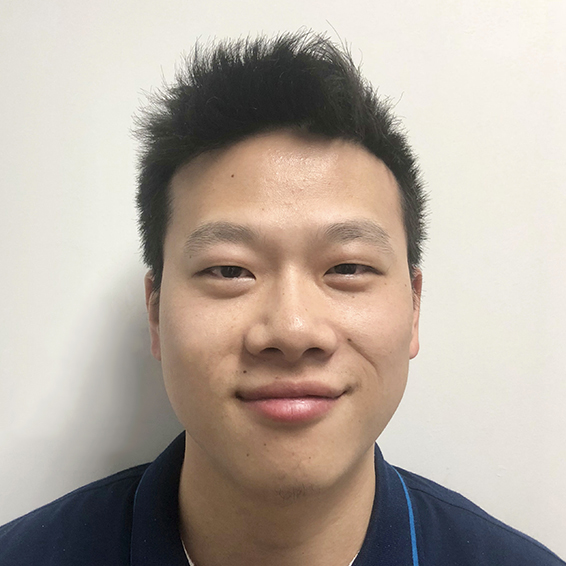
\includegraphics[height=2.7cm]{visa_photo.jpg}}
\end{tabular}
 \linebreak
%Section: Education

\section{\textbf{Education}}

\begin{tabular}{lc}
% \textbf{Institute of High Energy Physics, Chinese Academy of Science}  \\
% \hspace{1cm} PhD candidate in High Energy Astrophysics (Autumn 2020 diploma receive)\\



% Thesis title:"\textit{Study of the high-energy properties of pulsars observed by Insight-HXMT}"\\

\textbf{\textsc{Sept. 2015 -- Present}: Ph.D. candidate (Expected Autumn 2020)} \\
\hspace{2cm} Institute of High Energy Physics, Chinese Academy of Science
\\
\hspace{2cm} Thesis title: \textit{Study of the high-energy properties of pulsars}\\
\hspace{2cm} \textit{observed by Insight-HXMT} \\

\textbf{\textsc{Jun. 2011 -- Jun. 2015:} B.Sc. in Mathematics and Physics}\\
\hspace{2cm} Yunnan University, Kunming, China

\end{tabular}
\linebreak
%Section: Scholarships and additional info
\section{\textbf{Conference \& Workshop}}
\begin{tabular}{ll}
\textsc{Nov. } 2019: Beijing Astronomical Annual Meeting \hspace{4cm}| Bejing,China
\\ 
\hspace{2cm} \textbf{Oral Presentation (Award of best presentation)}
\\
\hspace{2cm} Title: \textit{Temporal study on HMXB 4U\,1901+03 observed by \textit{Insight}-HXMT} 
  \\
%------
\textsc{Jul. } 2019: The 8th Fermi Asian Network Workshop  \footnotesize{Fermi-LAT summer school for FAN8} \\
\hspace{13.5cm}| Zhuhai, China\normalsize
\\
%------
\textsc{Jun. } 2019: The Second Insight-HXMT Users Conference \hspace{2.7cm}| Beijing, China
\\
\hspace{2cm} \textbf{Oral Presentation} \normalsize\\
\hspace{2cm} Title: \textit{Timing and spectral analysis using Insight-HXMT data}\\
\hspace{2cm} \textbf{Lecturing the usage of Insight-HXMT data analysis software} \normalsize
\\
%------
\textsc{Dec. } 2018: Insight-HXMT Users Workshop \hspace{5cm}| Beijing, China\\
\hspace{2cm} \textbf{Oral Presentation}\\
\hspace{2cm} Title: \textit{Quick tour to Insight-HXMT/HE data processing}\\
\hspace{2cm} \textbf{Lecturing the usage of Insight-HXMT data analysis software} \normalsize
\\
%------
\textsc{Nov. } 2018: Japan China X-ray Collaboration Workshop \hspace{3cm}| Toyoko, Japan\\ 
\hspace{2cm} \textbf{Oral Presentation}\\
\hspace{2cm} Title: \textit{Insight-HXMT observations of newly discovered XRB Swift\,J0243.6+6124}
\\
%------
\textsc{Oct. } 2018: Annual Meeting of Chinese Astronomical Society \hspace{2cm}| Kunming, China
\\
\hspace{2cm} \textbf{Oral Presentation}\\
\hspace{2cm} Title: \textit{Insight-HXMT observations of Crab pulsar}
\\
%------
\textsc{Jul. } 2018: Summer School and Workshop for Nuclear Astrophysics \hspace{1cm}| Enshi, China
\\ 
%------
\textsc{Jul. } 2018: The 42nd COSPAR Scientific Assembly \hspace{4cm}| Pasadena, U.S. \\
\hspace{2cm} \textbf{Poster}\\
\hspace{2cm} Title: \textit{Insight-HXMT observations of newly discovered XRB Swift\,J0243.6+6124}\\

\end{tabular}

\section{\textbf{Computer Skills}}
\begin{tabular}{lr}
Data Analysis Packages:& \textsc{HXMTDAS} (\score{4.8}{5}) \\
& \textsc{xspec} (\score{4}{5})\\
& \textsc{ftools} (\score{4}{5})\\
& Analyzing experiences with \\
& NuSTAR, Fermi and MAXI \\
% & Data Plot:& \textsc{Python}\\%\setmainfont[SmallCapsFont=Fontin-SmallCaps.otf]{Fontin.otf}\\
% Operating System:& \textsc{Macos},\textsc{linux}&Typeset:& \textsc{{\fb \LaTeX}}\\
Scripting languages:& \textsc{python} (\score{4.5}{5}) \\
& \textsc{GNU bash} (\score{3}{5}) \\
Programming language:& \textsc{C++} (\score{1}{5})\\
% Typeset:& \textsc{{\fb \LaTeX}} (Intermediate)
\end{tabular}
\\
\\
GitLab link: \url{http://code.ihep.ac.cn/tuoyl} \\
GitHub link: \url{https://www.github.com/tuoyl}\\    


\section{\textbf{Developed Software Tools}}

\begin{tabular}{l l}
 \href{https://github.com/tuoyl/hxmt_docker}{HXMT Docker Container}: An integrated environment for \textit{Inishgt}-HXMT \\
 \hspace{4.8cm} data analysis\\
 %------
 \href{http://code.ihep.ac.cn/hxmthsdc/hxmt_pipeline}{HXMT pipeline}:\hspace{1.8cm} A pipeline tool that makes your life easier \\
 \hspace{4.8cm} when analyzing HXMT data\\
%-------
\href{https://github.com/tuoyl/HXMT_BurstAnalysis}{HXMT Burst Analysis}:\hspace{0.6cm} A supplementary toolkit for correcting the saturation effect \\
\hspace{4.8cm} of LE telespoce on-board HXMT\\
\href{https://github.com/tuoyl/CsI_analysis}{HXMT CsI Analysis}:\hspace{1cm} A script to search the pulsation signal of CsI detector \\
\hspace{4.8cm} on-board HXMT\\
\href{https://github.com/tuoyl/TimingAnalysis}{Timing Analysis toolkit}:\hspace{0.4cm} A toolkit for timing analysis of pulsar and binary
 
\end{tabular}



\newpage

\section{\textbf{Publication list}}
     \hspace{2cm}\\
\textbf{Published:}\\
\noindent\makebox[0.5\linewidth]{\rule{0.5\textwidth}{1pt}} \\
\pubbullet{}\textbf{Insight-HXMT insight into switch of the accretion mode: The case of the X-ray pulsar 4U 1901+03}
\begin{description}
\item \textcolor{blue}{\textit{\textbf{Y.L. Tuo}}}, L. Ji, S.S. Tsygankov, T. Mihara, L.M. Song, ..., and Insight-HXMT collaboration, 2020, Journal of High Energy Astrophysics, 27(38-43)
\end{description}

\pubbullet{}\textbf{Insight-HXMT observations of the Crab pulsar}
\begin{description}
\item \textcolor{blue}{\textit{\textbf{Y.L. Tuo}}}, M.Y.Ge, L.M. Song, L.L. Yan, Q.C.Bu, and J.L. Qu., 2019, Research of Astronomy and Astrophysics, 19(6), 087. 
\end{description}

\pubbullet{}\textbf{The Insight-HXMT observation of the newly discovered transient X-ray pulsar Swift\,J0243.6+6124}
\begin{description}
  \item \textcolor{blue}{\textit{\textbf{Y.L. Tuo}}}, and Y. Zhang., 42nd COSPAR Scientific Assembly. Vol. 42. 2018.
\end{description}

\pubbullet{}\textbf{Time evolution of the X-ray and gamma-ray fluxes of the Crab pulsar}
\begin{description}
\item L.L. Yan, M.Y. Ge, F.J. Lu, S.J. Zheng, \textcolor{blue}{\textit{\textbf{Y.L. Tuo}}}, Z.J. Li, J.L. Qu, 2018, The Astrophysical Journal , 865(1), 21.
\end{description}

\pubbullet{}\textbf{Phase Evolution of the Crab Pulsar between Radio and X-ray}
\begin{description}
  \item L.L. Yan, M.Y. Ge, J.P. Yuan, S.J. Zheng, F.J. Lu, \me{}, H. Tong, S. N. Zhang, Y. Lu, J.L. Han, and Y.J. Du, 2017, The Astrophysical Journal, 845(2), 119.
\end{description}

\hspace{2cm}\\
\textbf{In Process:}\\
\noindent\makebox[0.5\linewidth]{\rule{0.5\textwidth}{1pt}} \\
\pubbullet{}\textbf{Identification of a non-thermal X-ray burst with the Galactic magnetar SGR 1935+2154 and a fast radio burst with Insight-HXMT}
\begin{description}
  \item C.K. Li, L. Lin, S.L. Xiong, M.Y. Ge, X.B. Li, T.P. Li, F.J. Lu, S.N. Zhang, \me{}, ..., and the Insight-HXMT collaboration, (arXiV pre-print: https://arxiv.org/abs/2005.11071v1)
\end{description}

\pubbullet{}\textbf{The jet-like corona in a black hole X-ray binary observed by Insight-HXMT}
\begin{description}
  \item B. Y, \me{}, C.Z. Li, W. Wang, S.N. Zhang, S. Zhang, M.Y. Zhang, ... and the Insight-HXMT collaboration, (Revised and Resubmitted to Nature Communication)
\end{description}






%---------------------------------
\newpage
\section{Research Experience}
\setlength{\parindent}{2em}
\hspace{2cm}\par
% \textbf{\textsc{Pulsar Timing}}\\
My career as a Ph.D. student accompanied the launch and first three years of operation of the HXMT. I have participated in the in-flight calibration of HXMT, software development and maintenance, and some of the studies of its scientific targets, including pulsars, black holes, and the gamma-ray burst. I have experience in data analysis of timing and spectral of various astronomical sources. Moreover, I have developed tools to support the analysis of HXMT data. 

\large\textbf{\textsc{Observational studies of compact objects}}
\normalsize

\textbf{\textit{Insight-HXMT observations of the Crab pulsar}}

The Crab pulsar has been used in the calibration of multi-band astronomy instruments because of their stable and high luminosity, and relatively stable time characteristics. We used HXMT's observations in the first year after the launch of the Crab pulsar to perform the timing and spectral analysis. In terms of timing, we report timing residuals of less than $\SI{50}{\us}$ for HXMT observations of Crab pulsar, which verifies the correctness of the HXMT time system. A good time performance then allows the study of the pulse profiles of Crab pulsars. Since the HXMT covers a broad X-ray energy band, 1\,keV--250\,keV, we analyze the evolution of the pulse profile with energy and obtain the spectrum for each rotating phase. This work provides additional data on pulsars to help constrain emitting models in the hard X-ray energy band. The detailed observational study of Crab also provides data to support the calibration of the instrument's systematic errors, and the PSF calibration.

\textbf{\emph{Insight-HXMT insight into the switch of the Accretion mode: The case of the X-ray. pulsar 4U 1901+03}}

An important scientific goal of the HXMT is to study the behavior of X-ray binary star systems during their outbursts. 4U\,1901+03 is a binary system in which the central compact object is a neutron star. MAXI, \textit{Swift}/BAT, and \textit{Fermi} monitored this source during its 2019 outburst. HXMT has carried out observations during its outburst decline. Using data from HXMT and \textit{Fermi}/GBM, we analyzed the periodic evolution of its binary stars, updated the orbital parameters of the system, and rotation parameters of the neutron star.

We analyze the evolution of its pulse profile during the outburst. The X-ray luminosity of the accretion powered pulsar changes as the absorption rate changes. At the same time, changes of radiation pressure within the absorption column leads to a switch of the accreting mode, which also a variation in the shape of the pulse profile (varies between double and single peaks). We have observed changes in the pulse profile in both HXMT and NuSTAR data. From this, we can establish the correlation between bolometric luminosity and magnetic field, while the flux is known by observations. Thus the correlation between the distance and the magnetic can be obtained.

Meanwhile, the luminosity of the accretion powered pulsar corresponds to the variation of the accreting rate. The variation of the accretion rate is directly responsible for the effect of the accreted material on the acceleration of the neutron star's rotation ($\dot{\nu}$). Based on the torque model of the accreting process, we obtain the equation containing the $\dot{\nu}$, magnetic field, and the distance of the source. Since the optical observations of this source do not provide good constrain to the distance of this source, we suggest the distance of $12.5\pm0.2\,\rm{kpc}$, and the magnetic field of $4.3\times10^{12}\,\rm{G}$.

\newpage
\textbf{\emph{Spectroscopic study of the black hole binary MAXI\,J1820+070}}

I participated in a study of black hole X-ray binary MAXI\,J1820+070, contributing to spectral analysis and interpretation of results.
HXMT observations of MAXI\,J1820+070, covering a complete outburst of the source. Kara et al. (2019) suggested a reduction in the spatial extent of the corona during the hard-state of the black hole. A consequence of this process is that the proportion of photons reflected from the corona reaching the accretion disk increases as the flux decreases. Using data from HXMT, we find that the fraction from the reflected component is decreasing. We suggest that this is caused by the outflow from the corona. The main part of my contribution is the analysis of HXMT data as well as the spectral. The MCMC method is used to simulate the parameter in the parameter space. The credit intervals of the parameters are determined using the posterior distributions of the parameters. Because the height of the corona decreases physically, in the reflection model the corona height increases, we fit the responsed fake spectra by simulating a reflection model with an outflow in the velocity of $\beta$. The results confirm that the outflow leads to the height increasing of the corona in the model, which explains the observation well.





%\newpage
%\section{Research Plan}
%\hspace{2cm}\par
%My interest lies in several fields of X-ray astronomy, especially the X-ray timing and spectral studies of pulsars. Based on the researches I carried out theses years, some questions remain on the table.

%1) The pulsar's glitch and X-ray emission properties

%The recent results reported by PolarLight (H. Feng et al. 2020) show that the polarization fraction of the Crab in the on-pulse phases was observed to decrease after a glitch of the Crab pulsar on 23 July 2019, while the PWN properties remain unchanged. The variation in the polarization of the Crab pulsar during glitch may be caused by a change in the configuration of magnetic fields. We expect the change in the X-ray properties, for example, the shape change in pulse profiles or a change in the on-pulse flux of the pulsar. Using the satellite data in the X-ray band with good time resolution such as NICER, HXMT/LE, etc., may help us understand the physics of the magnetic field near the neutron star.

%\noindent Another intriguing result is that the spin-down rate transition related to the brightening of the PWN of PSR B0540-69 (M.Y. Ge et al. 2019). They report the spin-down rate increased $\sim$36\%, which corresponding to the increasing of the PWN flux, while the on-pulsed flux had no changes. A close look into the X-ray properties during changes in pulsar timing properties can help us understand the magnetic field of pulsars and PWNs.

%2) The emission properties of the accretion powered pulsar

%The timing and spectral characteristics of the accretion powered pulsar during its outburst stage reveal the magnetic properties and the interaction between the neutron star and the accretion materials. In Y.L Tuo et al. (2020), we established the correlation between the source distance and the magnetic field strength for the XRB 4u\,1901+03, and reported the distance in the terms that optical observation could not give the precise distance. Does the estimation of the distance and the magnetic field based on the torque model of the accretion process apply to other accretion powered pulsars?  If the method is universally applicable for accretion X-ray pulsar, a distance and magnetic field catalog for accretion X-ray pulsar could be established.

%3) Software development for the mission

%I have developed many tools for data analysis of HXMT, involving pulsar timing, spectral analysis, and instrument effects, to make people's life easier. I've always had a passion for developing software based on the understanding of the instrument to make data analysis and research more accessible and elegant to scientists.










\end{document}
